\documentclass[aspectratio=169]{beamer}
\usepackage{color,amsmath}
\usepackage{subfigure}
\usepackage{booktabs}
\usepackage{framed}
\usepackage{comment}

\def\vf{\vfill}

%%%%%%%%%%%%%%%%%%%%%%%%%%
\title[]{Human computation\\(05-03)}
\author[]{Matthew J. Salganik\\Department of Sociology\\Princeton University}
\date[]{Soc 596: Computational Social Science\\Fall 2016
\vfill
\begin{flushright}
\vspace{0.6in}

\includegraphics[width=0.1\textwidth]{figures/cc.png}
\end{flushright}
}
\begin{document}
%%%%%%%%%%%%%%%%%%%%%%%%%%
\frame{\titlepage}
%%%%%%%%%%%%%%%%%%%%%%%%%%
\begin{frame}

\begin{itemize}
\item Easy task, big scale
\pause
\item Humans better than computers
\pause
\item Can be combined with supervised learning
\pause
\item Increasingly important as we move from numeric survey data to working with text, images, movies, audio, etc.
\end{itemize}

\end{frame}
%%%%%%%%%%%%%%%%%%%%%%%%%%
\begin{frame}

\begin{center}
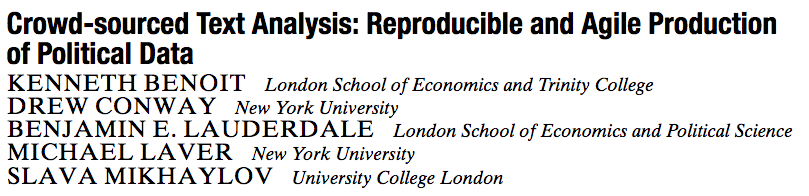
\includegraphics[width=\textwidth]{figures/benoit_crowd-sourced_2016_title}
\end{center}

\vf
{\tiny \url{http://dx.doi.org/10.1017/S0003055416000058}}

\end{frame}
%%%%%%%%%%%%%%%%%%%%%%%%%%
\begin{frame}

\begin{center}
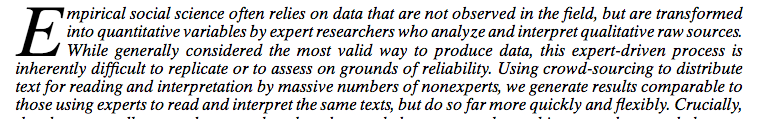
\includegraphics[width=\textwidth]{figures/benoit_crowd-sourced_2016_abstract}
\end{center}

\end{frame}
%%%%%%%%%%%%%%%%%%%%%%%%%%
\begin{frame}

\begin{itemize}
\item Better not cheaper
\pause
\item Experts are a bug not a feature
\end{itemize}

\end{frame}
%%%%%%%%%%%%%%%%%%%%%%%%%%
\begin{frame}

{\Large
\begin{center}
To Turk or not to Turk?
\end{center}
}

\end{frame}
%%%%%%%%%%%%%%%%%%%%%%%%%%
\begin{frame}

{\Large
\begin{center}
Questions?  Comments?  Ideas? Suggestions?
\end{center}
}

\end{frame}
%%%%%%%%%%%%%%%%%%%%%%%%%%

\end{document}
